\documentclass{article}

% content/resources/templates/preamble.tex
\usepackage[margin=0.6in]{geometry}
\author{Milav Dabgar}
\usepackage{amsmath,amssymb,amsthm}
\usepackage{booktabs}
\usepackage{multirow}
\usepackage{xcolor}
\usepackage{tcolorbox}
\tcbuselibrary{breakable,skins}
\usepackage[colorlinks=true,linkcolor=blue]{hyperref}
\usepackage{titlesec}
\usepackage{enumitem}
\usepackage{tikz}
\usepackage{pgfplots}
\usepackage{circuitikz}
\usepackage[version=4]{mhchem}
\usepackage{longtable}
\usepackage{array}
\usepackage{float}
\usepackage{caption}
\usepackage{listings}

\lstset{
  basicstyle=\small\ttfamily,
  breaklines=true,
  breakatwhitespace=false,
  postbreak=\mbox{\textcolor{red}{$\hookrightarrow$}\space},
  float=false,
  numbers=left,
  numberstyle=\tiny\color{gray},
  numbersep=10pt,
  xleftmargin=2em,
  keywordstyle=\color{blue},
  commentstyle=\color{green!60!black},
  stringstyle=\color{purple},
  backgroundcolor=\color{gray!5},
  showstringspaces=false,
  tabsize=2,
  captionpos=b,
  keepspaces=true,
  columns=flexible
}

\pgfplotsset{compat=1.18}
\usetikzlibrary{shapes,arrows,positioning,calc,patterns,decorations.pathmorphing,decorations.markings,arrows.meta}

% Color scheme
\definecolor{headcolor}{RGB}{0,102,204}
\definecolor{keycolor}{RGB}{220,20,60}
\definecolor{solutioncolor}{RGB}{34,139,34}
\definecolor{mnemoniccolor}{RGB}{148,0,211}
\definecolor{codecolor}{RGB}{0,0,100}

% Spacing
\setlength{\parskip}{3pt}
\setlist[itemize]{nosep}
\setlist[enumerate]{nosep}

% Title formatting
\titleformat{\section}{\Large\bfseries\color{headcolor}}{\thesection}{1em}{}
\titleformat{\subsection}{\large\bfseries\color{headcolor}}{\thesubsection}{1em}{}

% Pandoc tightlist compatibility
\providecommand{\tightlist}{%
  \setlength{\itemsep}{0pt}\setlength{\parskip}{0pt}}

% Pandoc longtable compatibility
\newcounter{none}
\def\thenone{}


% content/resources/templates/english-boxes.tex

% Custom environments
\newtcolorbox{solutionbox}{
 breakable,
 enhanced,
 colback=solutioncolor!5!white,
 colframe=solutioncolor!75!black,
 fonttitle=\bfseries,
 title=Solution
}

\newtcolorbox{solutionboxnobreak}{
 colback=solutioncolor!5!white,
 colframe=solutioncolor!75!black,
 fonttitle=\bfseries,
 title=Solution
}

\newtcolorbox{keyformula}{
 breakable,
 enhanced,
 colback=keycolor!5!white,
 colframe=keycolor!75!black,
 fonttitle=\bfseries,
 title=Key Formula
}

\newtcolorbox{mnemonicboxenv}{
 breakable,
 enhanced,
 colback=mnemoniccolor!5!white,
 colframe=mnemoniccolor!75!black,
 fonttitle=\bfseries,
 title=Mnemonic
}

\newcommand{\mnemonicbox}[1]{%
  \begin{mnemonicboxenv}
    #1
  \end{mnemonicboxenv}
}


% Custom commands for GTU solutions
% This file defines semantic commands for consistent formatting

% Question command with automatic formatting
\newcommand{\question}[2]{%
  \section*{Question #1}%
  \textbf{#2}%
}

% OR question variant
\newcommand{\questionor}[2]{%
  \section*{Question #1 OR}%
  \textbf{#2}%
}

% Proper table environment with caption
\newenvironment{answertable}[1]{%
  \begin{table}[htbp]
  \centering
  \caption{#1}
}{%
  \end{table}
}

% Proper figure environment for diagrams
\newenvironment{answerdiagram}[1]{%
  \begin{figure}[htbp]
  \centering
  \caption{#1}
}{%
  \end{figure}
}

% Semantic markup for key terms
\newcommand{\keyword}[1]{\textbf{#1}}
\newcommand{\code}[1]{\texttt{#1}}
\newcommand{\classname}[1]{\texttt{#1}}
\newcommand{\methodname}[1]{\texttt{#1}}

% Proper quotation marks
\newcommand{\mnemonic}[1]{``#1''}


\title{Data Structure with Python (4331601) - Summer 2024 Solution}
\date{June 06, 2024}

\begin{document}
\maketitle

\questionmarks{1(a)}{3}{Differentiate between array and list.}

\begin{solutionbox}
\textbf{Answer}:

\begin{center}
\captionof{table}{Array vs List}
\begin{tabulary}{\linewidth}{|L|L|}
\hline
\textbf{Array} & \textbf{List} \\
\hline
\textbf{Fixed size} at creation & \textbf{Dynamic size} - can grow/shrink \\
\hline
\textbf{Homogeneous} data (same type) & \textbf{Heterogeneous} data (mixed types) \\
\hline
\textbf{Memory efficient} - contiguous allocation & \textbf{Flexible} but uses more memory \\
\hline
\textbf{Faster access} for calculations & \textbf{Built-in methods} for operations \\
\hline
\end{tabulary}
\end{center}
\end{solutionbox}

\begin{mnemonicbox}
Arrays are Fixed Friends, Lists are Loose Leaders
\end{mnemonicbox}

\questionmarks{1(b)}{4}{Explain the concept of class and object with the help of python program.}

\begin{solutionbox}
\textbf{Answer}:

\keyword{Class} is a blueprint that defines the structure and behavior of objects. \keyword{Object} is an instance of a class.

\begin{lstlisting}[language=Python,caption={Class and Object Example}]
class Student:
    def __init__(self, name, age):
        self.name = name
        self.age = age
    
    def display(self):
        print(f"Name: {self.name}, Age: {self.age}")

# Creating objects
s1 = Student("Ram", 20)
s2 = Student("Sita", 19)
s1.display()
\end{lstlisting}

\begin{itemize}
    \item \keyword{Class}: Creates the Template
    \item \keyword{Object}: Creates the Real instance
    \item \keyword{Constructor}: Initializes the Object
\end{itemize}
\end{solutionbox}

\begin{mnemonicbox}
Class Blueprints Create Object Instances
\end{mnemonicbox}

\questionmarks{1(c)}{7}{Define constructor. Discuss different types of constructors with suitable python program.}

\begin{solutionbox}
\textbf{Answer}:

\keyword{Constructor} is a special method that is automatically called at object creation time. In Python, the \code{\_\_init\_\_()} method is the constructor.

\begin{lstlisting}[language=Python,caption={Constructor Types}]
class Demo:
    # Default Constructor
    def __init__(self):
        self.value = 0
    
    # Parameterized Constructor
    def __init__(self, x, y=10):
        self.x = x
        self.y = y

# Usage
d1 = Demo(5)      # x=5, y=10 (default)
d2 = Demo(3, 7)   # x=3, y=7
\end{lstlisting}

\textbf{Types of Constructors:}

\begin{center}
\captionof{table}{Types of Constructors}
\begin{tabulary}{\linewidth}{|L|L|L|}
\hline
\textbf{Type} & \textbf{Description} & \textbf{Usage} \\
\hline
\textbf{Default} & No parameters & Object initialization \\
\hline
\textbf{Parameterized} & With parameters & Custom initialization \\
\hline
\textbf{Copy} & Creates copy of object & Object duplication \\
\hline
\end{tabulary}
\end{center}
\end{solutionbox}

\begin{mnemonicbox}
Default Parameters Copy Objects
\end{mnemonicbox}

\questionmarks{1(c OR)}{7}{Define Polymorphism. Write a python program for polymorphism through inheritance.}

\begin{solutionbox}
\textbf{Answer}:

\keyword{Polymorphism} is the ability to perform different operations on different objects using the same interface.

\begin{lstlisting}[language=Python,caption={Polymorphism Example}]
class Animal:
    def sound(self):
        pass

class Dog(Animal):
    def sound(self):
        return "Woof!"

class Cat(Animal):
    def sound(self):
        return "Meow!"

# Polymorphic behavior
animals = [Dog(), Cat()]
for animal in animals:
    print(animal.sound())
\end{lstlisting}

\begin{itemize}
    \item \keyword{Method Overriding}: Same method name in Child class
    \item \keyword{Dynamic Binding}: Method selection at runtime
    \item \keyword{Code Reusability}: Same interface, different implementation
\end{itemize}
\end{solutionbox}

\begin{mnemonicbox}
Many Objects, One Interface
\end{mnemonicbox}

\questionmarks{2(a)}{3}{Explain Python specific data structure List, Tuple and Dictionary.}

\begin{solutionbox}
\textbf{Answer}:

\begin{center}
\captionof{table}{List vs Tuple vs Dictionary}
\begin{tabulary}{\linewidth}{|L|L|L|}
\hline
\textbf{Data Structure} & \textbf{Properties} & \textbf{Example} \\
\hline
\textbf{List} & Mutable, ordered, allows duplicates & \code{[1, 2, 3, 2]} \\
\hline
\textbf{Tuple} & Immutable, ordered, allows duplicates & \code{(1, 2, 3, 2)} \\
\hline
\textbf{Dictionary} & Mutable, key-value pairs, no duplicate keys & \code{\{'a': 1, 'b': 2\}} \\
\hline
\end{tabulary}
\end{center}
\end{solutionbox}

\begin{mnemonicbox}
Lists Change, Tuples Stay, Dictionaries Map
\end{mnemonicbox}

\questionmarks{2(b)}{4}{Explain application of stack.}

\begin{solutionbox}
\textbf{Answer}:

\textbf{Stack Applications:}

\begin{itemize}
    \item \keyword{Function Calls}: Call stack management
    \item \keyword{Expression Evaluation}: Infix to postfix conversion
    \item \keyword{Undo Operations}: Text editors, browsers
    \item \keyword{Parentheses Matching}: Syntax checking
\end{itemize}

\begin{center}
\begin{tikzpicture}
    \node[gtu block, minimum width=2cm] (top) at (0,2) {3};
    \node[right] at (top.east) {$\leftarrow$ Top};
    \node[gtu block, minimum width=2cm] (mid) at (0,1) {2};
    \node[gtu block, minimum width=2cm] (bot) at (0,0) {1};
    
    \draw[thick] (-1.2,-0.5) -- (1.2,-0.5); % Base
    \draw[thick] (-1.2,-0.5) -- (-1.2,2.5); % Left wall
    \draw[thick] (1.2,-0.5) -- (1.2,2.5);   % Right wall
\end{tikzpicture}
\captionof{figure}{Stack Structure}
\end{center}
\end{solutionbox}

\begin{mnemonicbox}
Functions Evaluate Undo Parentheses
\end{mnemonicbox}

\questionmarks{2(c)}{7}{Define stack. Explain PUSH \& POP operation with example. Write an algorithm for PUSH and POP operations of stack.}

\begin{solutionbox}
\textbf{Answer}:

\keyword{Stack} is a linear data structure following the LIFO (Last In First Out) principle.

\textbf{PUSH Algorithm:}

\begin{enumerate}
    \item Check if stack is full
    \item If full, print "Stack Overflow"
    \item Else, increment top
    \item Add element at top position
\end{enumerate}

\textbf{POP Algorithm:}

\begin{enumerate}
    \item Check if stack is empty
    \item If empty, print "Stack Underflow"
    \item Else, remove element from top
    \item Decrement top
\end{enumerate}

\textbf{Example:}

\begin{lstlisting}[language=Python,caption={Stack Operations}]
stack = []
stack.append(10)  # PUSH
stack.append(20)  # PUSH
item = stack.pop()  # POP returns 20
\end{lstlisting}
\end{solutionbox}

\begin{mnemonicbox}
Last In, First Out - Like Plates
\end{mnemonicbox}

\questionmarks{2(a OR)}{3}{Define Following terms: I. Time Complexity II. Space Complexity III. Best case}

\begin{solutionbox}
\textbf{Answer}:

\begin{center}
\captionof{table}{Complexity Terms}
\begin{tabulary}{\linewidth}{|L|L|L|}
\hline
\textbf{Term} & \textbf{Definition} & \textbf{Example} \\
\hline
\textbf{Time Complexity} & Algorithm execution time analysis & $O(n)$, $O(\log n)$ \\
\hline
\textbf{Space Complexity} & Memory usage analysis & $O(1)$, $O(n)$ \\
\hline
\textbf{Best Case} & Minimum time/space needed & Sorted array search \\
\hline
\end{tabulary}
\end{center}
\end{solutionbox}

\begin{mnemonicbox}
Time Space Best Performance
\end{mnemonicbox}

\questionmarks{2(b OR)}{4}{Convert A – (B / C + (D \% E * F) / G)* H into postfix expression}

\begin{solutionbox}
\textbf{Answer}:

\textbf{Step-by-step conversion:}

\begin{itemize}
    \item Infix: $A - (B / C + (D \% E * F) / G) * H$
    \item Result: $A\ B\ C\ /\ D\ E\ \%\ F\ *\ G\ /\ +\ -\ H\ *$
\end{itemize}

\textbf{Stack operations:}
\begin{itemize}
    \item Operators: $-, (, /, +, (, \%, *, ), /, ), *$
    \item Final: \code{A B C / D E \% F * G / + - H *}
\end{itemize}

\textbf{Postfix Result:} \code{A B C / D E \% F * G / + - H *}
\end{solutionbox}

\begin{mnemonicbox}
Operands First, Operators Follow
\end{mnemonicbox}

\questionmarks{2(c OR)}{7}{Define circular queue. Explain INSERT and DELETE operations of circular queue with diagrams.}

\begin{solutionbox}
\textbf{Answer}:

\keyword{Circular Queue} is a modified version of a queue where the last position is connected to the first position.

\begin{center}
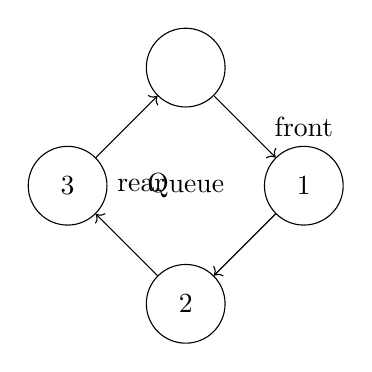
\begin{tikzpicture}
    \foreach \i in {1,2,3,4} {
        \node[draw, circle, minimum size=1cm] (n\i) at ({90-90*\i}:1.5) {\ifnum\i=4 \else \i \fi};
    }
    \draw[->] (n1) -- (n2);
    \draw[->] (n2) -- (n3);
    \draw[->] (n3) -- (n4);
    \draw[->] (n4) -- (n1);
    
    \node at (0,0) {Queue};
    \node[above] at (n1.north) {front};
    \node[right] at (n3.east) {rear};
\end{tikzpicture}
\captionof{figure}{Circular Queue}
\end{center}

\textbf{INSERT Algorithm:}

\begin{enumerate}
    \item Check if queue is full
    \item rear = (rear + 1) \% size
    \item queue[rear] = element
    \item If first element, set front = 0
\end{enumerate}

\textbf{DELETE Algorithm:}

\begin{enumerate}
    \item Check if queue is empty
    \item element = queue[front]
    \item front = (front + 1) \% size
    \item Return element
\end{enumerate}

\begin{itemize}
    \item \keyword{Advantage}: Memory efficiency
    \item \keyword{Application}: CPU scheduling, buffering
\end{itemize}
\end{solutionbox}

\begin{mnemonicbox}
Circle Back When Full
\end{mnemonicbox}

\questionmarks{3(a)}{3}{Explain Implementation of Stack using List.}

\begin{solutionbox}
\textbf{Answer}:

Stack operations using Python List:

\begin{lstlisting}[language=Python,caption={Stack using List}]
stack = []  # Empty stack
stack.append(10)  # PUSH
stack.append(20)  # PUSH
top = stack.pop()  # POP
\end{lstlisting}

\begin{itemize}
    \item \keyword{PUSH}: \code{append()} method
    \item \keyword{POP}: \code{pop()} method
    \item \keyword{TOP}: \code{stack[-1]} for peek
\end{itemize}
\end{solutionbox}

\begin{mnemonicbox}
Append Pushes, Pop Pulls
\end{mnemonicbox}

\questionmarks{3(b)}{4}{Discuss different applications of linked list.}

\begin{solutionbox}
\textbf{Answer}:

\textbf{Linked List Applications:}

\begin{itemize}
    \item \keyword{Dynamic Memory}: Size varies at runtime
    \item \keyword{Insertion/Deletion}: Efficient at any position
    \item \keyword{Implementation}: Stacks, queues, graphs
    \item \keyword{Undo Functionality}: Browser history, text editors
\end{itemize}

\begin{center}
\captionof{table}{Linked List Applications}
\begin{tabulary}{\linewidth}{|L|L|L|}
\hline
\textbf{Application} & \textbf{Advantage} & \textbf{Use Case} \\
\hline
\textbf{Music Playlist} & Easy add/remove & Media players \\
\hline
\textbf{Memory Management} & Dynamic allocation & Operating systems \\
\hline
\textbf{Polynomial Representation} & Efficient storage & Mathematical operations \\
\hline
\end{tabulary}
\end{center}
\end{solutionbox}

\begin{mnemonicbox}
Dynamic Implementation Undo Memory
\end{mnemonicbox}

\questionmarks{3(c)}{7}{Explain doubly linked list. Write an algorithm to delete a node from the beginning of doubly linked list}

\begin{solutionbox}
\textbf{Answer}:

\keyword{Doubly Linked List} has nodes containing data, next pointer, and previous pointer.

\begin{center}
\begin{tikzpicture}[gtu box]
    \node[draw, rectangle split, rectangle split parts=3, rectangle split horizontal] (n1) {prev \nodepart{second} data \nodepart{third} next};
    \node[below=0.2cm] at (n1.one south) {NULL};
    \draw[->] (n1.one south) -- (n1.one);
    
    \node[below=0.2cm] at (n1.three south) {next};
    \draw[->] (n1.three) -- (n1.three south);
\end{tikzpicture}
\captionof{figure}{Doubly Linked List Node}
\end{center}

\textbf{Delete from Beginning Algorithm:}

\begin{enumerate}
    \item If list is empty, return
    \item If only one node:
    \begin{itemize}
        \item head = NULL
    \end{itemize}
    \item Else:
    \begin{itemize}
        \item temp = head
        \item head = head.next
        \item head.prev = NULL
        \item delete temp
    \end{itemize}
\end{enumerate}

\begin{lstlisting}[language=Python,caption={Delete from Beginning}]
def delete_beginning(self):
    if self.head is None:
        return
    if self.head.next is None:
        self.head = None
    else:
        self.head = self.head.next
        self.head.prev = None
\end{lstlisting}
\end{solutionbox}

\begin{mnemonicbox}
Two Way Navigation
\end{mnemonicbox}

\questionmarks{3(a OR)}{3}{Convert this Infix expression into Postfix expression: A+B/C*D-E/F-G}

\begin{solutionbox}
\textbf{Answer}:

\textbf{Step-by-step conversion:}

\begin{itemize}
    \item Infix: $A+B/C*D-E/F-G$
    \item Postfix: $A\ B\ C\ /\ D\ *\ +\ E\ F\ /\ -\ G\ -$
    \item Operator precedence: $*, / > +, -$
    \item Left to right associativity
\end{itemize}
\end{solutionbox}

\begin{mnemonicbox}
Multiply Divide Before Add Subtract
\end{mnemonicbox}

\questionmarks{3(b OR)}{4}{Explain Circular Linked List with its disadvantages.}

\begin{solutionbox}
\textbf{Answer}:

In \keyword{Circular Linked List}, the last node's next pointer points to the first node.

\begin{center}
\begin{tikzpicture}[gtu box]
    \node[gtu block] (n1) at (0,0) {1};
    \node[gtu block] (n2) at (2,0) {2};
    \node[gtu block] (n3) at (4,0) {3};
    
    \draw[gtu arrow] (n1) -- (n2);
    \draw[gtu arrow] (n2) -- (n3);
    \draw[gtu arrow] (n3.south) -- ++(0,-0.5) -| (n1.south);
\end{tikzpicture}
\captionof{figure}{Circular Linked List}
\end{center}

\textbf{Disadvantages:}

\begin{itemize}
    \item \keyword{Infinite Loop Risk}: Improper traversal
    \item \keyword{Complex Implementation}: Extra care needed
    \item \keyword{Memory Overhead}: Additional pointer management
    \item \keyword{Debugging Difficulty}: Circular references
\end{itemize}
\end{solutionbox}

\begin{mnemonicbox}
Circles Can Cause Confusion
\end{mnemonicbox}

\questionmarks{3(c OR)}{7}{Write a Python Program to perform Insert operation in doubly Linked List. Explain with neat diagrams.}

\begin{solutionbox}
\textbf{Answer}:

\begin{lstlisting}[language=Python,caption={Insert in Doubly Linked List}]
class Node:
    def __init__(self, data):
        self.data = data
        self.next = None
        self.prev = None

class DoublyLinkedList:
    def __init__(self):
        self.head = None
    
    def insert_beginning(self, data):
        new_node = Node(data)
        if self.head is None:
            self.head = new_node
        else:
            new_node.next = self.head
            self.head.prev = new_node
            self.head = new_node
\end{lstlisting}

\begin{center}
\begin{tikzpicture}[gtu box]
    \node[draw, rectangle split, rectangle split parts=3, rectangle split horizontal] (n1) at (0,0) {prev \nodepart{second} 10 \nodepart{third} next};
    \node[draw, rectangle split, rectangle split parts=3, rectangle split horizontal] (n0) at (-3,0) {prev \nodepart{second} 5 \nodepart{third} next};
    
    \draw[gtu arrow] (n0.three) -- (n1.one);
    \draw[gtu arrow] (n1.one) to[bend left] (n0.three);
    
    \node[below] at (n0.south) {New Head};
\end{tikzpicture}
\captionof{figure}{Inserting New Head}
\end{center}

\textbf{Insert Operations:}

\begin{itemize}
    \item \keyword{Beginning}: Update head pointer
    \item \keyword{End}: Traverse to last node
    \item \keyword{Middle}: Update prev/next pointers
\end{itemize}
\end{solutionbox}

\begin{mnemonicbox}
Begin End Middle Insertions
\end{mnemonicbox}

\questionmarks{4(a)}{3}{Write an algorithm for Merge sort.}

\begin{solutionbox}
\textbf{Answer}:

\textbf{Merge Sort Algorithm:}

\begin{enumerate}
    \item If array size $\le$ 1, return
    \item Divide array into two halves
    \item Recursively sort both halves
    \item Merge sorted halves
\end{enumerate}

\textbf{Time Complexity}: $O(n \log n)$ \\
\textbf{Space Complexity}: $O(n)$
\end{solutionbox}

\begin{mnemonicbox}
Divide Conquer Merge
\end{mnemonicbox}

\questionmarks{4(b)}{4}{Differentiate between Singly Linked List and Doubly Linked List.}

\begin{solutionbox}
\textbf{Answer}:

\begin{center}
\captionof{table}{Singly vs Doubly Linked List}
\begin{tabulary}{\linewidth}{|L|L|}
\hline
\textbf{Singly Linked List} & \textbf{Doubly Linked List} \\
\hline
\textbf{One pointer} (next) & \textbf{Two pointers} (next, prev) \\
\hline
\textbf{Forward traversal} only & \textbf{Bidirectional traversal} \\
\hline
\textbf{Less memory} usage & \textbf{More memory} usage \\
\hline
\textbf{Simple implementation} & \textbf{Complex implementation} \\
\hline
\end{tabulary}
\end{center}

\begin{center}
\begin{tikzpicture}[gtu box]
    \node (singly) at (0,1) {Singly: [data|next] $\rightarrow$ NULL};
    \node (doubly) at (0,0) {Doubly: NULL $\leftarrow$ [prev|data|next] $\leftrightarrow$ [prev|data|next] $\rightarrow$ NULL};
\end{tikzpicture}
\captionof{figure}{Linked List Types}
\end{center}
\end{solutionbox}

\begin{mnemonicbox}
Single Forward, Double Bidirectional
\end{mnemonicbox}

\questionmarks{4(c)}{7}{Write an algorithm for selection sort. Give the trace to sort the given data using selection sort method. Data are: 13, 2, 6, 54, 18, 42, 11}

\begin{solutionbox}
\textbf{Answer}:

\textbf{Selection Sort Algorithm:}

\begin{enumerate}
    \item For i = 0 to n-2:
    \item Find minimum in array[i...n-1]
    \item Swap minimum with array[i]
    \end{enumerate}

\textbf{Trace for [13, 2, 6, 54, 18, 42, 11]:}

\begin{center}
\captionof{table}{Selection Sort Trace}
\begin{tabulary}{\linewidth}{|C|C|C|C|}
\hline
\textbf{Pass} & \textbf{Array State} & \textbf{Min Found} & \textbf{Swap} \\
\hline
0 & [13, 2, 6, 54, 18, 42, 11] & 2 & 13$\leftrightarrow$2 \\
\hline
1 & [2, 13, 6, 54, 18, 42, 11] & 6 & 13$\leftrightarrow$6 \\
\hline
2 & [2, 6, 13, 54, 18, 42, 11] & 11 & 13$\leftrightarrow$11 \\
\hline
3 & [2, 6, 11, 54, 18, 42, 13] & 13 & 54$\leftrightarrow$13 \\
\hline
4 & [2, 6, 11, 13, 18, 42, 54] & 18 & No swap \\
\hline
5 & [2, 6, 11, 13, 18, 42, 54] & 42 & No swap \\
\hline
\end{tabulary}
\end{center}

\textbf{Final Result: [2, 6, 11, 13, 18, 42, 54]}
\end{solutionbox}

\begin{mnemonicbox}
Select Minimum, Swap Position
\end{mnemonicbox}

\questionmarks{4(a OR)}{3}{Write an algorithm for Insertion sort.}

\begin{solutionbox}
\textbf{Answer}:

\textbf{Insertion Sort Algorithm:}

\begin{enumerate}
    \item For i = 1 to n-1:
    \item key = array[i]
    \item j = i-1
    \item While j >= 0 and array[j] > key:
    \item \quad array[j+1] = array[j]
    \item \quad j = j-1
    \item array[j+1] = key
\end{enumerate}

\textbf{Time Complexity}: $O(n^2)$ \\
\textbf{Best Case}: $O(n)$ for sorted array
\end{solutionbox}

\begin{mnemonicbox}
Insert In Right Position
\end{mnemonicbox}

\questionmarks{4(b OR)}{4}{Write an algorithm to insert a new node at the end of circular linked list.}

\begin{solutionbox}
\textbf{Answer}:

\textbf{Algorithm:}

\begin{enumerate}
    \item Create new\_node with data
    \item If list is empty:
    \begin{itemize}
        \item head = new\_node
        \item new\_node.next = new\_node
    \end{itemize}
    \item Else:
    \begin{itemize}
        \item temp = head
        \item While temp.next != head:
        \item \quad temp = temp.next
        \item temp.next = new\_node
        \item new\_node.next = head
    \end{itemize}
\end{enumerate}

\begin{lstlisting}[language=Python,caption={Insert at End Circular Linked List}]
def insert_end(self, data):
    new_node = Node(data)
    if self.head is None:
        self.head = new_node
        new_node.next = new_node
    else:
        temp = self.head
        while temp.next != self.head:
            temp = temp.next
        temp.next = new_node
        new_node.next = self.head
\end{lstlisting}
\end{solutionbox}

\begin{mnemonicbox}
Circle Back To Head
\end{mnemonicbox}

\questionmarks{4(c OR)}{7}{Write an algorithm for bubble sort. Give the trace to sort the given data using bubble sort method. Data are: 37, 22, 64, 84, 58, 52, 11}

\begin{solutionbox}
\textbf{Answer}:

\textbf{Bubble Sort Algorithm:}

\begin{enumerate}
    \item For i = 0 to n-2:
    \item For j = 0 to n-2-i:
    \item If array[j] > array[j+1]:
    \item \quad Swap array[j] and array[j+1]
\end{enumerate}

\textbf{Trace for [37, 22, 64, 84, 58, 52, 11]:}

\begin{center}
\captionof{table}{Bubble Sort Trace}
\begin{tabulary}{\linewidth}{|C|L|L|}
\hline
\textbf{Pass} & \textbf{Comparisons \& Swaps} & \textbf{Result} \\
\hline
1 & 37$\leftrightarrow$22, 64$\leftrightarrow$84, 84$\leftrightarrow$58, 84$\leftrightarrow$52, 84$\leftrightarrow$11 & [22, 37, 64, 58, 52, 11, 84] \\
\hline
2 & 37$\leftrightarrow$64, 64$\leftrightarrow$58, 64$\leftrightarrow$52, 64$\leftrightarrow$11 & [22, 37, 58, 52, 11, 64, 84] \\
\hline
3 & 37$\leftrightarrow$58, 58$\leftrightarrow$52, 58$\leftrightarrow$11 & [22, 37, 52, 11, 58, 64, 84] \\
\hline
4 & 37$\leftrightarrow$52, 52$\leftrightarrow$11 & [22, 37, 11, 52, 58, 64, 84] \\
\hline
5 & 37$\leftrightarrow$11 & [22, 11, 37, 52, 58, 64, 84] \\
\hline
6 & 22$\leftrightarrow$11 & [11, 22, 37, 52, 58, 64, 84] \\
\hline
\end{tabulary}
\end{center}

\textbf{Final Result: [11, 22, 37, 52, 58, 64, 84]}
\end{solutionbox}

\begin{mnemonicbox}
Bubble Up The Largest
\end{mnemonicbox}

\questionmarks{5(a)}{3}{Explain Binary search tree and application of it.}

\begin{solutionbox}
\textbf{Answer}:

\keyword{Binary Search Tree (BST)} is a binary tree where the left subtree contains smaller values and the right subtree contains larger values.

\textbf{Properties:}

\begin{itemize}
    \item \keyword{Left child} $<$ \keyword{Parent} $<$ \keyword{Right child}
    \item \keyword{Inorder traversal} gives sorted sequence
    \item \keyword{Search time}: $O(\log n)$ average case
\end{itemize}

\textbf{Applications:}

\begin{center}
\captionof{table}{BST Applications}
\begin{tabulary}{\linewidth}{|L|L|L|}
\hline
\textbf{Application} & \textbf{Benefit} & \textbf{Use Case} \\
\hline
\textbf{Database Indexing} & Fast search & DBMS systems \\
\hline
\textbf{Expression Trees} & Evaluation & Compilers \\
\hline
\textbf{Huffman Coding} & Compression & Data compression \\
\hline
\end{tabulary}
\end{center}
\end{solutionbox}

\begin{mnemonicbox}
Binary Search Trees Organize Data
\end{mnemonicbox}

\questionmarks{5(b)}{4}{Write Python Program for Linear Search and explain it with an example}

\begin{solutionbox}
\textbf{Answer}:

\begin{lstlisting}[language=Python,caption={Linear Search}]
def linear_search(arr, target):
    for i in range(len(arr)):
        if arr[i] == target:
            return i
    return -1

# Example
numbers = [10, 25, 30, 45, 60]
result = linear_search(numbers, 30)
print(f"Element found at index: {result}")  # Output: 2
\end{lstlisting}

\textbf{Working:}

\begin{itemize}
    \item \keyword{Sequential check}: Element by element
    \item \keyword{Time Complexity}: $O(n)$
    \item \keyword{Space Complexity}: $O(1)$
    \item \keyword{Works on}: Unsorted arrays
\end{itemize}

\begin{center}
\captionof{table}{Linear Search Trace}
\begin{tabulary}{\linewidth}{|L|L|L|}
\hline
\textbf{Step} & \textbf{Element} & \textbf{Found?} \\
\hline
1 & 10 & No \\
\hline
2 & 25 & No \\
\hline
3 & 30 & Yes! \\
\hline
\end{tabulary}
\end{center}
\end{solutionbox}

\begin{mnemonicbox}
Linear Line By Line
\end{mnemonicbox}

\questionmarks{5(c)}{7}{Create a Binary Search Tree for the keys 45, 35, 12, 58, 5, 55, 58, 80, 35, 42 and write the Preorder, Inorder and Postorder traversal sequences.}

\begin{solutionbox}
\textbf{Answer}:

\textbf{BST Construction (duplicates ignored):}

\begin{center}
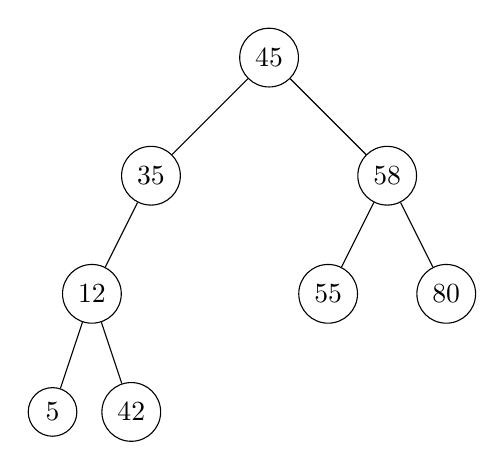
\begin{tikzpicture}[
    level 1/.style={sibling distance=3cm},
    level 2/.style={sibling distance=1.5cm},
    level 3/.style={sibling distance=1cm}]
    
    \node[circle, draw] {45}
        child {node[circle, draw] {35}
            child {node[circle, draw] {12}
                child {node[circle, draw] {5}}
                child {node[circle, draw] {42}}
            }
            child[missing]
        }
        child {node[circle, draw] {58}
            child {node[circle, draw] {55}}
            child {node[circle, draw] {80}}
        };
\end{tikzpicture}
\captionof{figure}{Binary Search Tree}
\end{center}

\textbf{Insertion Order:} 45(root), 35(left), 12(left of 35), 58(right), 5(left of 12), 55(left of 58), 80(right of 58), 42(right of 12)

\textbf{Traversals:}

\begin{center}
\captionof{table}{Traversals}
\begin{tabulary}{\linewidth}{|L|L|L|}
\hline
\textbf{Traversal} & \textbf{Sequence} & \textbf{Rule} \\
\hline
\textbf{Preorder} & 45, 35, 12, 5, 42, 58, 55, 80 & Root-Left-Right \\
\hline
\textbf{Inorder} & 5, 12, 35, 42, 45, 55, 58, 80 & Left-Root-Right \\
\hline
\textbf{Postorder} & 5, 42, 12, 35, 55, 80, 58, 45 & Left-Right-Root \\
\hline
\end{tabulary}
\end{center}
\end{solutionbox}

\begin{mnemonicbox}
Pre-Root First, In-Sorted, Post-Root Last
\end{mnemonicbox}

\questionmarks{5(a OR)}{3}{Define following terms: I. Binary tree II. level number III. Leaf-node}

\begin{solutionbox}
\textbf{Answer}:

\begin{center}
\captionof{table}{Binary Tree Terms}
\begin{tabulary}{\linewidth}{|L|L|L|}
\hline
\textbf{Term} & \textbf{Definition} & \textbf{Example} \\
\hline
\textbf{Binary tree} & Tree with max 2 children per node & Each node has $\le$ 2 children \\
\hline
\textbf{Level number} & Distance from root (root = level 0) & Root=0, children=1, etc. \\
\hline
\textbf{Leaf-node} & Node with no children & Terminal nodes \\
\hline
\end{tabulary}
\end{center}

\begin{center}
\begin{tikzpicture}[gtu box]
    \node[circle, draw] (a) at (0,0) {A};
    \node[circle, draw] (b) at (-1,-1) {B};
    \node[circle, draw] (c) at (1,-1) {C};
    \node[circle, draw] (d) at (-1.5,-2) {D};
    
    \draw (a) -- (b);
    \draw (a) -- (c);
    \draw (b) -- (d);
    
    \node[right] at (a.east) {$\leftarrow$ Root (L0)};
    \node[right] at (c.east) {$\leftarrow$ L1};
    \node[right] at (d.east) {$\leftarrow$ Leaf (L2)};
\end{tikzpicture}
\captionof{figure}{Binary Tree Levels}
\end{center}
\end{solutionbox}

\begin{mnemonicbox}
Binary Levels Lead To Leaves
\end{mnemonicbox}

\questionmarks{5(b OR)}{4}{Differentiate between Linear Search and Binary search.}

\begin{solutionbox}
\textbf{Answer}:

\begin{center}
\captionof{table}{Linear vs Binary Search}
\begin{tabulary}{\linewidth}{|L|L|}
\hline
\textbf{Linear Search} & \textbf{Binary Search} \\
\hline
\textbf{Works on unsorted} arrays & \textbf{Requires sorted} array \\
\hline
\textbf{Sequential checking} & \textbf{Divide and conquer} \\
\hline
\textbf{Time}: $O(n)$ & \textbf{Time}: $O(\log n)$ \\
\hline
\textbf{Simple implementation} & \textbf{Complex implementation} \\
\hline
\textbf{No preprocessing} needed & \textbf{Sorting required} \\
\hline
\end{tabulary}
\end{center}

\begin{center}
\begin{tikzpicture}[gtu box]
    \node[align=left] at (0,1) {Linear: Check 1, Check 2, ...};
    \node[align=left] at (0,0) {Binary: Check Middle, Ignored Half};
\end{tikzpicture}
\captionof{figure}{Search Comparison}
\end{center}
\end{solutionbox}

\begin{mnemonicbox}
Linear Line, Binary Bisect
\end{mnemonicbox}

\questionmarks{5(c OR)}{7}{Write an algorithm for insertion and deletion a node in Binary search tree.}

\begin{solutionbox}
\textbf{Answer}:

\textbf{Insertion Algorithm:}

\begin{enumerate}
    \item If root is NULL, create new node as root
    \item If data $<$ root.data, insert in left subtree
    \item If data $>$ root.data, insert in right subtree
    \item If data == root.data, no insertion (duplicate)
\end{enumerate}

\textbf{Deletion Algorithm:}

\begin{enumerate}
    \item If node is leaf: Simply delete
    \item If node has one child: Replace with child
    \item If node has two children:
    \begin{itemize}
        \item Find inorder successor
        \item Replace data with successor's data
        \item Delete successor
    \end{itemize}
\end{enumerate}

\begin{lstlisting}[language=Python,caption={BST Operations}]
def insert(root, data):
    if root is None:
        return Node(data)
    if data < root.data:
        root.left = insert(root.left, data)
    elif data > root.data:
        root.right = insert(root.right, data)
    return root

def delete(root, data):
    if root is None:
        return root
    if data < root.data:
        root.left = delete(root.left, data)
    elif data > root.data:
        root.right = delete(root.right, data)
    else:
        # Node to be deleted found
        if root.left is None:
            return root.right
        elif root.right is None:
            return root.left
        # Node with two children
        temp = find_min(root.right)
        root.data = temp.data
        root.right = delete(root.right, temp.data)
    return root
\end{lstlisting}

\textbf{Cases:}

\begin{itemize}
    \item \keyword{Leaf deletion}: Direct removal
    \item \keyword{One child}: Replace with child
    \item \keyword{Two children}: Replace with successor
\end{itemize}
\end{solutionbox}

\begin{mnemonicbox}
Insert Compare, Delete Replace
\end{mnemonicbox}

\end{document}
